\documentclass[handout,12pt]{beamer}
\usepackage{pgfpages}
\pgfpagesuselayout{4 on 1}[a4paper,landscape,border shrink=5mm]

\usepackage[latin1]{inputenc}
\usepackage[english]{babel}
\usepackage{epsfig}
\usepackage{rotating}
\usepackage{graphicx}
%\usepackage{mslapa}
\usepackage{amsmath}
%\usepackage[all]{xy}
% \usepackage{amssymb,graphicx}
%\input psfig.sty
\usepackage{booktabs}
\usepackage{graphpap}
\usepackage{verbatim}
%\usepackage{amsbsy}
\graphicspath{{C:/Users/janne.pitkaniemi/figures/}}

\setbeamertemplate{footline}[page number]
\DeclareGraphicsExtensions{.pdf, .jpg, .png,.jpeg}
% \DeclareGraphicsExtensions{.eps}

\newcommand{\Rlogo}[1]{
\includegraphics[#1]{Rlogo}}
\newcommand{\RSlogo}[1]{\includegraphics[#1]{RStudio-logo}}

% This is a file of useful extra commands snatched from
% Michael Hills, David Clayton, Bendix Carstensen & Esa Laara.
%

% Commands to draw observation lines on follow-up diagrams
%
% Horizontal lines
%

% exit time with failure, bullet
\newcommand{\hfail}[1]{\begin{picture}(250,5)
       \put(0,0){\line(0,1){2.5}}
      \put(0,0){\line(0,-1){2.5}}
      \put(0,0){\line(1,0){#1}}
      \put(#1,0){\circle*{5}}
   \end{picture}}

% exit time with censoring, open circle
\newcommand{\hcens}[1]{\begin{picture}(250,5)
         \put(0,0){\line(0,1){2.5}}
      \put(0,0){\line(0,-1){2.5}}
      \put(0,0){\line(1,0){#1}}
%      \put(#1,0){\line(0,1){2.5}}
%      \put(#1,0){\line(0,-1){2.5}}
% BxC Changed this to an open circle instead of a line
      \put(#1,0){\circle{5}}
   \end{picture}}

%
% Diagonals for Lexis diagrams
%
\newcommand{\dfail}[1]{\begin{picture}(250,250)
      \put(0,0){\line(1,1){#1}}
      \put(#1,#1){\circle*{5}}
   \end{picture}}

\newcommand{\dcens}[1]{\begin{picture}(250,250)
      \put(0,0){\line(1,1){#1}}
%      \put(#1,#1){\line(0,1){2.5}}
%      \put(#1,#1){\line(0,-1){2.5}}
% BxC Changed this to an open circle instead of a line
      \put(#1,#1){\circle{5}}
   \end{picture}}

%
% Horizontal range diagrams
%
\newcommand{\hrange}[1]{\begin{picture}(200,5)
     \put(0,0){\circle*{5}}
     \put(0,0){\line(1,0){#1}}
     \put(0,0){\line(-1,0){#1}}
   \end{picture}}

%
% Tree drawing
%
\newcommand{\tree}[3]{\setlength{\unitlength}{#1}\begin{picture}(0,0)
   \put(0,0){\line(3,2){1}}
   \put(0,0){\line(3,-2){1}}
   \put(0.81,0.54){\makebox(0,0)[br]{\footnotesize #2\ }}
   \put(0.81,-0.54){\makebox(0,0)[tr]{\footnotesize #3\ }}
\end{picture}}

\newcommand{\wtree}[3]{\setlength{\unitlength}{#1}\begin{picture}(0,0)
   \put(0,0){\line(1,1){1}}
   \put(0,0){\line(1,-1){1}}
   \put(0.8,0.8){\makebox(0,0)[br]{\footnotesize #2\ }}
   \put(0.8,-0.8){\makebox(0,0)[tr]{\footnotesize #3\ }}
\end{picture}}

\newcommand{\ntree}[3]{\setlength{\unitlength}{#1}\begin{picture}(0,0)
   \put(0,0){\line(2,1){1}}
   \put(0,0){\line(2,-1){1}}
   \put(0.8,0.4){\makebox(0,0)[br]{\footnotesize #2\ }}
   \put(0.8,-0.4){\makebox(0,0)[tr]{\footnotesize #3\ }}
\end{picture}}

%
% Other commands
%
\newcommand{\prob}[0]{\text{\rm Pr}}
\newcommand{\nhy}[0]{_{\oslash}}
\newcommand{\true}[0]{_{\text{\rm \tiny T}}}
\newcommand{\hyp}[0]{_{\text{\rm \tiny H}}}
% \newcommand{\mpydiv}[0]{\stackrel{\textstyle \times}{\div}}
% Changed to slightly smaller symbols
\newcommand{\mpydiv}[0]{\stackrel{\times}{\scriptstyle \div}}
\newcommand{\mie}[1]{{\it #1}}
\newcommand{\mycircle}[0]{\circle*{5}}
\newcommand{\smcircle}[0]{\circle*{1}}
\newcommand{\corner}[0]{_{\text{\rm \tiny C}}}
\newcommand{\ind}[0]{\hspace{10pt}}
\newcommand{\gap}[0]{\\[5pt]}
\renewcommand{\S}[0]{section~}
\newcommand{\blank}[0]{$\;\,$}
\newcommand{\vone}{\vspace{1cm}}
\newcommand{\ljust}[1]{\multicolumn{1}{l}{#1}}
\newcommand{\cjust}[1]{\multicolumn{1}{c}{#1}}
\newcommand{\mean}{\text{\rm Mean}}
\newcommand{\transpose}{^{\mbox{\tiny T}}}
\newcommand{\histog}[5]{\rule{1mm}{#1mm}\,\rule{1mm}{#2mm}\,\rule{1mm}{#3mm}\,\rule{1mm}{#4mm}\,\rule{1mm}{#5mm}}
\newcommand{\pmiss}{P_{\mbox{\tiny miss}}}
%
% Below is BxCs commands inserted
%
\newcommand{\bc}{\begin{center}}
\newcommand{\ec}{\end{center}}

\newcommand{\bd}{\setlength{\parskip}{1ex} \begin{description}}
\newcommand{\ed}{\end{description} \setlength{\parskip}{2ex}}
\newcommand{\bdx}{\begin{description}} % Bendix' description macros
\newcommand{\edx}{\end{description}}

\newcommand{\bix}{\begin{itemize}}  % these are Bendix' itemizing macros
\newcommand{\eix}{\end{itemize}}
\newcommand{\bi}{\setlength{\parskip}{1ex} \begin{itemize}} % Esa's item macros 
\newcommand{\ei}{\end{itemize} \setlength{\parskip}{2ex}} 

\newcommand{\bn}{\begin{equation}}
\newcommand{\en}{\end{equation}}
\newcommand{\be}{\begin{enumerate}}
\newcommand{\ee}{\end{enumerate}}
\newcommand{\bes}{\begin{eqnarray*}}
\newcommand{\ees}{\end{eqnarray*}}
\newcommand{\p}{\text{\rm P}}
\newcommand{\pmat}[1]{\text{\rm P}\left\{#1\right\}}
\newcommand{\ptxt}[1]{\text{\rm P}\left\{\text{\rm #1}\right\}}
\newcommand{\E}{\text{\rm E}}
\newcommand{\V}{\text{\rm V}}
\newcommand{\BLUP}{\text{\rm BLUP}}

% \newcommand{\var}{\mbox{Var}} changed by Esa to
\newcommand{\var}{\mbox{var}}
% \newcommand{\cov}{\mbox{Cov}} changed by Esa to
\newcommand{\cov}{\mbox{cov}}
% \newcommand{\corr}{\mbox{Corr}} changed by Esa to
\newcommand{\corr}{\mbox{corr}} 

%\newcommand{\var}{\text{\rm var}}
%\newcommand{\cov}{\text{\rm cov}}
%\newcommand{\corr}{\text{\rm corr}}
\newcommand{\se}{\text{\rm s.e.}}
\newcommand{\sd}{\text{\rm std}}
\newcommand{\erf}{\text{\rm erf}}
\newcommand{\odds}{\text{\rm odds}}
\newcommand{\bin}{\text{\rm binom}}
\newcommand{\half}[1]{\frac{1}{#1}}
% \newcommand{\td}[0]{\stackrel{\textstyle \times}{\div}}
% Changed to slightly smaller symbols
\newcommand{\td}[0]{\stackrel{\scriptstyle \times}{\scriptstyle \div}}
\newcommand{\logit}{\text{\rm logit}}
\newcommand{\link}{\text{\rm link}}
\newcommand{\spn}{\text{\rm span}}
\newcommand{\OR}{\text{\rm OR}}
\newcommand{\CI}{\text{\rm CI}}
\newcommand{\RR}{\text{\rm RR}}
\newcommand{\QR}{\text{\rm QR}}
\newcommand{\QD}{\text{\rm QD}}
\newcommand{\ER}{\text{\rm ER}}
\newcommand{\EM}{\text{\rm EM}}
\newcommand{\EF}{\text{\rm EF}}
\newcommand{\RD}{\text{\rm RD}}
\newcommand{\AC}{\text{\rm AC}}
\newcommand{\AF}{\text{\rm AF}}
\newcommand{\PAF}{\text{\rm PAF}}
\newcommand{\SR}{\text{\rm SR}}
\newcommand{\SMR}{\text{\rm SMR}}
\newcommand{\SEL}{\text{\rm SEL}}
\newcommand{\CMF}{\text{\rm CMF}}
\newcommand{\pvp}{\text{\rm PV}$+$}
\newcommand{\pvn}{\text{\rm PV}$-$}
\newcommand{\R}{\textsf{R}}
%\newcommand{\gap}[0]{\\[5pt]} 
%\newcommand{\blank}[0]{$\;\,$}
% Conditional independence sign from Philip Dawid
\newcommand{\cip}{\mbox{$\perp\!\!\!\perp$}}

%%% Commands to comment out parts of the text
\newcommand{\GLEM}[1]{}
\newcommand{\FORGETIT}[1]{}
\newcommand{\OMIT}[1]{}

%%% Insert output from program in small text 
%%% (requires package verbatim)

\newcommand{\insout}[1]{
\scriptsize
\renewcommand{\baselinestretch}{0.8}
\verbatiminput{#1}
\renewcommand{\baselinestretch}{1.0}
\normalsize
}

% From Esa:        
\newcommand{\T}{\text{\rm \small{T}}}
\newcommand{\id}{\text{\rm id}}
\newcommand{\Dev}{\text{\rm Dev}}
\newcommand{\Bin}{\text{\rm Bin}}
\newcommand{\probit}{\text{\rm probit}}
\newcommand{\cloglog}{\text{\rm cloglog}}
%\newcommand{\EF}{\text{\rm EF}}
\newcommand{\SE}{\text{\rm SE}}
\newcommand{\IP}{\text{\rm IP}}
\newcommand{\+}{\tiny +}


\usepackage[labelformat=empty]{caption}
\captionsetup[figure]{labelformat=empty}

% \newcommand{\R}{\bf \textsf{R}}
\parskip\medskipamount



\title{Epidemiologic Data Analysis using R\\
Part 1: Introduction}  % : \\ Analysis of Follow-up Studies}
%
\includegraphics[width=1\textwidth]{Rlogo.png}
% \Rlogo{height=1em} }

\author{Janne Pitk\"aniemi \\ (Esa L{\"a}{\"a}r{\"a})}

\institute{Finnish Cancer Registry, Finland,   
 \texttt{<janne.pitkaniemi@cancer.fi>} \\
 (University of Oulu, Finland,   
 \texttt{<esa.laara@oulu.fi>}) }

\date{Tampere University, Faculty of Social Sciences \newline % University of Tampere/Postgraduate training,
{\footnotesize Feb 26 - Mar 9,  2018} }

%\begin{center} \Rlogo{height=2em} \end{center}

\AtBeginSubsection[]
{
  \begin{frame}<beamer>
    \frametitle{Outline}
    \tableofcontents[currentsection,currentsubsection]
  \end{frame}
}

%\beamerdefaultoverlayspecification{<+->}

\begin{document}
\definecolor{darkgreen}{rgb}{0,.5,0}

\begin{frame}
    \titlepage
\end{frame}



%-------------------------------------------

\begin{frame}
\frametitle{Contents \Rlogo{height=1.2em}}
\ \\
\bi
\item[1.] Basic properties of R
\medskip
\item[2.] Script files
\medskip
\item[3.] Data structures and objects
\medskip
\item[4.] Data input and output
\medskip
\item[5.] Functions
\medskip
\item[6.] Tabulation functions
\ei
\end{frame}

\begin{frame}
\frametitle{What is \Rlogo{height=1.2em}?}
%\pause

\begin{itemize}
\item Statistical software % or ''package'' 
    --- and a lot more \pause\medskip
\item R is a {\bf language} and {\bf environment} for
      statistical computing and graphics 
      (\texttt{\small www.r-project.org/}) \pause\medskip
\item Developed by % an international community of 
   volunteers, coordinated by the \\ % lead by 
    \textbf{R Development Core Team}. \pause\medskip
\item Available for Windows, Linux, Mac, Unix, \dots. \pause\medskip 
\item Is expanding rapidly: new version every 6 months. \pause\medskip  
\item No licence fee(!) \& source code open. \pause\medskip
\end{itemize}
For further information and download: {\small\tt http://www.r-project.org/} 
\end{frame}


\begin{frame}
\frametitle{Properties of \Rlogo{height=1.2em}}

\pause
\bi
\item Large repertory of basic and advanced methods. \pause\medskip 
\item Versatile graphics of high quality. \pause\medskip 
\item % \Rlogo{height=0.8em}
 Reads datasets from Stata, SAS, SPSS, Epi-Info\\
 -- \ even Excel \pause\medskip
\item Deals simultaneously with different % \textit{objects} or \\
   data structures \\ -- \ not just a single data matrix. \pause\medskip 
\item Results of analysis saved as {\bf objects}, \\ 
     readily available for further processing. \pause\medskip 
\item Parsimonious output listing! \pause\medskip 
\item For advanced users! Easy to expand and tailor to specific needs
    using the \textbf{object-oriented} % available 
    programming tools. \medskip 
\ei
% \pause

% S  and R  have ''forever altered how people analyze, 
% visualize and manipulate data'' (John Chambers 1998)

\end{frame}

%---------------------------------------------

\begin{frame}[fragile]
\frametitle{To learn more about \Rlogo{height=2.2em}}
\ \\

% \medskip
% Oksanen, J. {\it R: Opas ekologeille.} 
% Biologian laitos, Oulun yliopisto, 2002.
% \texttt{http://cc.oulu.fi/$\sim$jarioksa/opetus/}
\begin{itemize}
\item
Hills, M., Plummer, M., Carstensen, B. \\
{\it A Short Introduction to R for Epidemiology}, 2011.
\small
 \verb|http://bendixcarstensen.com/Epi/R-intro.pdf|
\normalsize

\medskip
\item
Dalgaard, P. {\it Introductory Statistics with R, 2nd Ed.}\\
Springer, New York, 2008.

\pause\medskip
% Carstensen B. et al.
\item
 {\it Statistical Practice in Epidemiology Using R}.  
 An international course, IARC, Lyon, Jun 14-20, 2018.
 \small
\verb|http://bendixcarstensen.com/SPE/|
\normalsize
\item R blog
\small
\pause\medskip
\item
Documentation at the R home page: \verb|www.r-project.org/|

\pause\medskip
\item
Masses of  books, articles, websites, etc \dots
\end{itemize}

\end{frame}

%--------------------------------------------

\begin{frame}
\frametitle{What does \Rlogo{height=1.2em}\ offer for epidemiologists?}

\pause
\bi
\item Descriptive tools
\bi 
\item[--] Versatile tabulation
\item[--] High-quality graphics
\ei
\pause
\item Analytic methods
\bi
\item[--] Basic epidemiologic statistics
\item[--] Generalized linear models and their extensions
\item[--] Survival analysis methods
\item[--] Other \dots
\ei
\ei
\pause
These are provided by SAS and Stata, too, so why R \dots? 

\pause\medskip
Many features of R
are more appealing in the long run.
\end{frame}  

%---------------------------------------
\begin{frame}
\frametitle{Graphics in \Rlogo{height=1.2em}}

\bi
\item Versatile, flexible, high quality, \dots \pause\medskip
% \item Various {\bf high-level} graphic functions available. \pause\medskip
\item Easy to add items (points, lines, text, legends \dots) \\ %  \pause\medskip
to an existing graph. % by {\bf low-level} plotting commands. 
\pause\medskip
\item Fine tuning of symbols, lines, axes, colours, etc. by \\
 {\bf graphical parameters}  
  ($>$ 67 of them!) 
\pause\medskip
% \item Interactive tools
\item Interactive tools using the mouse
    \bi
    \item[--] Put new things on a graph 
    \item[--] Identify points 
    \ei
% : {\tt locator(); identify()}. 
\pause % \medskip 
\item Modern lattice or {\it Trellis} graphics % : package {\tt lattice}. \pause\medskip
% \item Saving formats:	
% Metafile, .pdf, .png, .bmp, .jpg, \dots
\ei
\end{frame}


\begin{frame}
\frametitle{Age-period-cohort incidence in DK}
\begin{figure}
\centering
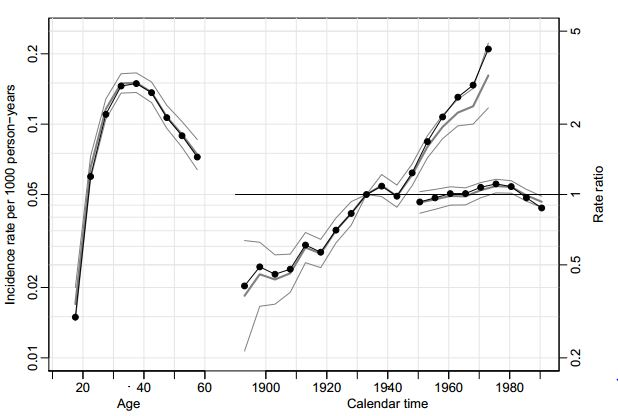
\includegraphics[width=0.8\linewidth]{APC_testis_cancer_dk}
\end{figure}
\end{frame}

\begin{frame}
\frametitle{Cancer predictions - Finland}
\begin{figure}
\centering
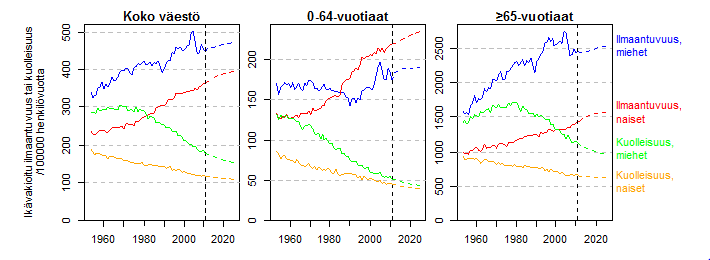
\includegraphics[width=1.1\linewidth]{Cancer_Finland}
\end{figure}
\end{frame}


\begin{frame}
\frametitle{Follow-up of Welsh nickel cohort in Lexis diagram}
\begin{figure}
\centering
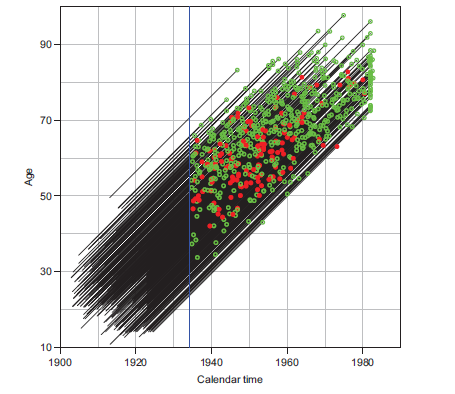
\includegraphics[width=0.8\linewidth]{Welsh}
\end{figure}
\end{frame}

\begin{frame}
\frametitle{RRs \& CIs by exposure in a cohort study}
\begin{figure}
\centering
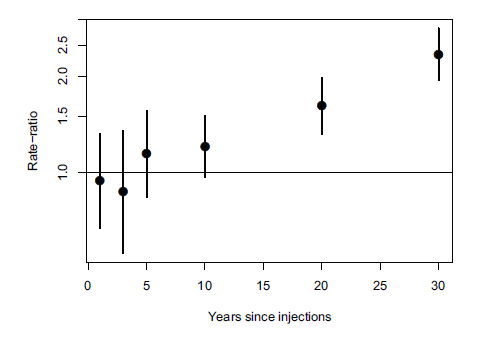
\includegraphics[width=1.0\linewidth]{RR-CI}
\end{figure}
\end{frame}

%%%%%%%%%%%%%%%%%%%%%%%%%%%%%%%%%%%%%%%%%%%%%%%%%%%%%%%%%%%%%%%%%%

 \begin{frame}
 \frametitle{Getting your graphs out}
 \ \\
 
 Graphs can be saved to disk % and later fetch them into your documents
 in almost any format % you like:
 \bi
 \item
 \texttt{.eps}, \texttt{.pdf}, \texttt{.bmp}, \texttt{.jpg}, 
 \texttt{.png}, \dots
 \ei
 
 \pause
 \bigskip
 Save graphs from the screen or write directly to
 a file.
 
  \pause\bigskip
 You can also directly transport an R graph as a metafile into a Word document!
\end{frame}

%-----------------------

\begin{frame}\frametitle{Package or library}
\ \\
\bi
\item Collection of functions pertaining to some 
    specialized application area, \emph{e.g.}
     {\tt survival, boot}
    \medskip
\item Contributed by users of R.
    \medskip
\item Available after loading:\\
	{\tt > library(survival)  }
	  \medskip
\item Alternatively load from the menu bar: \\
 {\it Packages - Load package... - Select one} 
   \medskip
\item New versions easily updated from Internet.
(https://www.rdocumentation.org/trends)
\ei
\end{frame}  

\begin{frame}
\frametitle{What does \Rlogo{height=1.2em}\ offer for epidemiologists?}

\pause
\bi
\item Descriptive tools
\bi 
\item[--] Versatile tabulation
\item[--] High-quality graphics
\ei
\pause
\item Analytic methods
\bi
\item[--] Basic epidemiologic statistics
\item[--] Generalized linear models and their extensions
\item[--] Survival analysis methods
\item[--] Other \dots
\ei
\ei
\pause
These are provided by SAS and Stata, too, so why R \dots? 

\pause\medskip
Many features of R
are more appealing in the long run.
\end{frame}  

%---------------------------------------
\begin{frame}[fragile]
\frametitle{R script -- R Studio -- commands in a file}

\ \\
\textbf{R script file} is an ASCII file
containing a sequence of R commands to be executed.

\bigskip
The {\bf script editor} -- use R-Studio \RSlogo{height=2.2em}
\bi
\item[1.] In {\tt R-Studio} open the script editor window: {\it New file - R script}, or when editing an existing {script file}:
 {\it File - Recent Files}, 
\pause\medskip
\pause\medskip    
\item[2.]    Save the {script file}: 
    {\it Save} \emph{e.g.} or     {\it Save As } {\tt *.R}
\item[3.]  Excecute a line {\it Ctrl-Enter}
    
\ei
\end{frame}

\begin{frame}[fragile]
\frametitle{R script (cont'd)}
\bi
 \item[4.] Paint the lines to be excecuted and {\it Ctrl -Enter} will execute lines.
 \pause\medskip  
\ei
 To run a whole script file, write in console window: \\
 {\tt > source("c:/.../mycmds.R", echo=TRUE)}

The script can also be written and edited by any external editor
programs (like Notepad). 

\end{frame}
%---------------------------------------

\begin{frame}\frametitle{Data objects of different kinds}

\bi
\item {\tt vector}: ordered set of similar elements \\ \emph{e.g.}
  real numbers or character sequences,
  \pause\medskip
\item {\tt factor}: categorical variable with levels \\ 
\emph{e.g.}
{\tt gender}, levels: {\tt c(1,2)} or {\tt c('male', 'female')}; 
\pause\medskip
\item {\tt matrix, array}: 2- and k-dimensional tables,
\pause\medskip
\item {\tt data.frame}: ``data matrix'' (more of this soon!),
\pause\medskip
\item {\tt ts}: time series object,
\pause\medskip
\item {\tt list}: sequence of different types of objects.
% \item {\tt function, expression}, \ldots
\ei
\end{frame}

%---------------------------------------% 

\begin{frame}\frametitle{Attributes of data objects}
\ \\
Functions that extract some key properties
of objects:
\bi 
\item {\tt length( )}: number of elements, 
\pause\medskip
\item {\tt mode( )}: basic type of elements, 
\pause\medskip
\item {\tt dim( )}: dimensions of arrays, matrices
   and data frames,
  \pause\medskip 
\item {\tt str( )}: overall structure, 
\pause\medskip
\item {\tt class( )}: property that determines
 how certain \\
 {\bf generic functions} (\emph{e.g.} 
 {\tt summary(); plot()}) \\
 work when the object is given as argument.
% \item {\tt name}: 
\ei
\end{frame}


\begin{frame}
\frametitle {Data frame -- data matrix}

\bd
\item[Data frame] = a {\bf list} of column vectors
\ed
\bi
% \item Formally a  % , all of equal length.
\item Rows correspond to observational units, and \\ columns (same length) refer to variables.
\pause\medskip
\item Column vectors can be \\ {\tt numeric, character} or {\tt logical}
\pause\medskip
\item Columns are \textbf{subobjects} of the data frame. Their \\
names are not directly accessible. Two possibilities:
\bi
 \item[(i)] Use ``surname\$firstname'', e.g. {\tt mydata\$var1}, 
 \pause\medskip
 \item[(ii)] Place the data frame in the search path at position 2: 
  {\tt attach(mydata)}; then use just ``firstname'': {\tt var1}
\ei
\ei
\end{frame}

\begin{frame}[fragile]
\frametitle{Data frame import from external files}

\bi
\item Common ASCII files, for example: \\
 \small 
\begin{verbatim}
   read.table("C:/owndir/rfiles/mydata.txt", ... );
   read.table("http://cc.oulu.fi/~tilel/esan.txt",...)
\end{verbatim}    
 \normalsize
\pause 
\item Files with fixed-width format: {\tt read.fwf()};
\pause\medskip
\item Files created in SPSS, SAS, Stata \emph{etc.}: 
functions \\
$\quad$ {\tt read.spss(), read.ssd(), read.dta()}, \emph{etc.} \\
in package {\tt foreign},
 \pause\medskip 
\item Excel-files: either {\tt read.table("clipboard", ...)}, or\\
 $\quad$ (1)\ save the Excel-file in {\tt .csv} or {\tt .txt} format, \\
 $\quad$ (2)\ in R: {\tt read.csv2( )} or {\tt read.table( )}
% \item Files from an Internet-address: function {\tt url( )}.
 \pause\medskip 
\item Relational DBMSs:  several R packages available.
\ei
\end{frame}

\begin{frame}[fragile]
\frametitle{Data frame import from external files with  \RSlogo{height=2.2em}}

Choose {\it Import Datasets} 

\bi
\item[ ] 
\pause 
\item[1.] {\it from text (base)} for \textbf{text} files
\item[2.] {\it from text (readr)} for \textbf{csv} files
\vspace*{0.3cm}
\item[3.] {\it from excel} for \textbf{excel} files
\vspace*{0.3cm}
\item[4.] {\it from SPSS} for \textbf{spss} files
\item[5.] {\it from SAS} for \textbf{sas} files
\item[6.] {\it from STATA} for \textbf{stata} files
\ei
\end{frame}

\begin{frame}\frametitle{Dealing with output}
\bi
\item The console contents, \emph{i.e.} the flow of input commands and output results 
from the console window, can be \\
$ \ \ - \ \ $ printed on paper: {\it File - Print...} \\
$ \ \ - \ \ $ saved to an ASCII file: {\it File - Save to file...}
\pause\medskip
\item Selected parts can be copied from the console and pasted to an external file.
\pause\medskip
\item
Function {\tt sink("results.txt")} diverts 
all subsequent output to an external text file.
Back to console: {\tt sink()}.
\pause\medskip
\item Choose {it\ New File -- R Markdown} output to MS-Word
\pause\medskip
\item Graphs saved in desired format: {\it File - Save...}  
\ei
\end{frame}


\begin{frame}\frametitle{R is a functional language}
\ \\

Most computations in R involve the {invocation} or {call} of functions.  They are called by name with a set of arguments separated by commas, \emph{e.g.} {\tt fun(x, y, z) ;} 

  {\bf Function} \\ 
  \bi
  \item[=] sequence of rules on how to produce 
    desired output: 
   \item[ ] {\bf value} of the function, 
    from given input, {\it i.e.} 
   \item[ ] {\bf arguments} of the function.
 \ei
 
\emph{Example}: Function {\tt sqrt()} computes square roots:

\medskip
{\tt > x <- c(0,1,2,3,4)  \#} argument vector defined\\
{\tt > sqrt(x)\ \ \ \ \#} call with argument {\tt x}; value printed:\\
{\tt [1] 0.000 1.000 1.414 1.732 2.000}
 
\end{frame} 

%----------------------------

\begin{frame}\frametitle{Defining a new function (1)}
\ \\
{\it Example}. Function {\tt CIapp} to calculate an approximate confidence interval
 from point estimate ({\tt estim}) 
and std error ({\tt SE}) by formula {\tt estim} $\pm$ $z_{\gamma/2}\ \times$ {\tt SE}. 

\medskip
Defining code (without prompts): \\
\ \\
{\tt CIapp <- function(estim, SE, level = 0.95) \{ \\
 \ \ \ z <- qnorm(1- (1-level)/2 )  \# setting the quantile\\
 \ \ \ lower <- estim - z*SE ; upper <- estim + z*SE  \\
 \ \ \ CIapp <- c(lower, upper)   \\
 \ \ \ CIapp \} 
}
\bi
\item {\bf Formal arguments}, here {\tt estim, SE, level}
\ei
\end{frame} 
%----------------------
\begin{frame}\frametitle{Calling the new function (1)}
% \ \\
\bi
\item {\bf Actual arguments}, used in function call: \\
{\tt > CIapp(3, 1, 0.9) \#} 90\% limits: $3 \pm 1.645\times 1$ \\
{\tt $[1]$ 1.355  4.645 }\\
\medskip
    NB! {\bf Positional matching}: order of actual arguments.
    \medskip
\item {\bf Keyword matching}: the order of arguments in the call is 
    irrelevant if the names of formal arguments are  given \\
	{\tt > CIapp(SE=1.0, level=0.90, estim=3)  }
	\medskip
\item If a {\bf default value} for an argument is given in the definition and is OK, it can be omitted in calling \\
{\tt > CIapp(3, 1) \#} 95\% limits: $3 \pm 1.96 \times 1$  \\
{\tt $[1]$ 1.040  4.960 }
\ei
\end{frame} 


%---------------------------------------------------

\begin{frame}\frametitle{Function call \& value object}
\bi
\item[(a)]
Simple call: Evaluates the value of the function with given arguments
and prints value items (according to  the print \textbf{method} specific to
  the \textbf{class} of the value object).
  \medskip
\item[(b)] Call of function and assignment of its value to an object.
\ei    
To extract information \& items from the value object, \emph{e.g.} 
\bi
\item {\tt str()}: overall structure,
\item {\tt names()}: names of the components,
\item {\tt print()}: selective printing of value items,
\item {\tt summary()}: selective print (not available for all functions).
% \item {\tt plot()}: certain graphical display, -"-    
\ei

\end{frame} 

%-----------------------------------------------------------

\begin{frame}\frametitle{Example, function {\tt range()}}
\ \\
Returns the minimum and maximum values
of a data vector.

{\tt > y <- c(15.3, 10.8, 8.1, 19.5, 5.3)  \#} data vector \\
\medskip
{\tt > range(y) \ \#} simple call with argument {\tt y}\\
{\tt [1]  5.3 19.5}\\
\medskip
{\tt > ra <- range(y) \#} call with assignment of value\\ 
\medskip
{\tt > ra \ \ \   \#} or {\tt print(ra)}, equivalent to simple call\\
{\tt [1]  5.3 19.5}\\
\medskip
{\tt > str(ra) \   \#} structure of the value object\\
{\tt num [1:2] 5.3 19.5}\\
\medskip
{\tt > ra[1]  \ \ \#} extracting an item from the value object\\
{\tt [1] 5.3}
\end{frame} 

%------------------------------------------------------


%---------------------------------------------------------

\begin{frame}\frametitle{Different kinds of functions} 
\bi
\item Mathematical, \emph{e.g.} {\tt sqrt(x); log(x); exp(x)}.\\
Arguments and values typically numeric vectors.
\medskip
\item
Data handling, \emph{e.g.} \\
{\tt dafr <- data.frame(x, y); \\
adata <- read.table("a.dat", header=T, ...); \\ % 
redc1 <- subset(redc, group == "24 h");}\\
Main argument(s): data object(s). Value: data object.
\medskip
\item 
Graphical, \emph{e.g.} \\
{\tt plot(y $\sim$ x); stripchart(y, xlim=c(0,3))} \\  
Main argument(s): data object(s). Value: graph. \\
Ancillary arguments: \emph{e.g.} graphical parameters.
\ei
\end{frame} 

%----------------------------------------------------

% \begin{comment}
\begin{frame}\frametitle{Value of the function}
\bi
\item numeric object (\emph{e.g.} vector, matrix) for many \\
  mathematical and statistical functions,
  \medskip
\item data object (e.g. vector, data frame) for \\ data handling functions,
\medskip
\item graph for graphical functions,
\medskip
\item table for tabulating functions,
\medskip
\item {\bf list} = a sequence of objects of different kinds, for \\
many statistical functions.
\ei
\end{frame} 
% \end{comment}
%--------------------------------------------------------------

\begin{frame}\frametitle{Statistical functions}
\bi
\item   {\it Main} argument(s): Typically data object(s). \\
        Often a {\it model formula}
        like {\tt y $\sim$ x} with \\ {\tt y} representing 
        the \emph{response} variable and \\
        expression {\tt x} = \emph{explanatory} variable(s) or factor(s).
        \medskip
\item
  \emph{Ancillary} arguments or \emph{parameters}: additional specifications.
    Some default values usually offered for these.
    \medskip
\item
  {\it Value}: Usually a {list} object consisting of several
  components of different types. %-- Note however graphics functions.
\ei
%    Example (ks. vanha luentomoniste, t.test)
\end{frame} 

%---------------------------------------------------------

\begin{frame}\frametitle{Function values as list objects}

\bi
\item {\bf List} = object consisting of an ordered collection of component objects, 
maybe of different types.
\medskip
\item
Provides a convenient way to return the \\
results of statistical computation.
\medskip
\item
A list with named components formed from existing objects: \\
\small 
${ }\quad $ {\small\tt Lista <- list(name=obj1,title=obj2,addr=obj3)} \\
\normalsize
A single component identified: \\
${ } \quad$ {\small\tt Lista{\$}name};
\medskip
\item
Concatenation of several lists into one: \\
${ }\quad$ \small  {\tt longlist <- c(list1, list2, \dots)}.
\normalsize
\ei
\end{frame} 

%---------------------------------------------------

\begin{frame}[fragile]
\frametitle{Ex: Function {\tt t.test()}}

\ \\
Description of syntax in the {\tt help()} page
\small
\begin{verbatim}
## Default S3 method:
t.test(x, y = NULL,
  alternative = c("two.sided", "less", "greater"), mu = 0,
  paired = FALSE, var.equal = FALSE, conf.level = 0.95, ...)
     
## S3 method for class 'formula':
  t.test(formula, data, subset, na.action, ...)
\end{verbatim}
\normalsize
\begin{itemize}
\item
Main argument(s): data vector(s) {\tt x} (and {\tt y}) or formula
\item
Ancillary arguments, like {\tt var.equal, conf.level}: \\
Default values given. 
\item
{\bf NB.} Dots '{\tt ...}'
\end{itemize}
\end{frame} 


%------------------------------------------------

\begin{frame}[fragile]
\frametitle{Example. Red cell folate levels}

 The data describe red cell folate levels (variable \texttt{folate},
$\mu$g/l) in two groups  
of cardiac bypass surgery patients given two different 
nitrous oxide ventilation (50\% NO + 50\% O$_2$) treatments
(variable \texttt{group}):
\begin{itemize}
\item
group 1 ($n_1 = 8$)
continuously for 24 h (label \texttt{"24 h"}),
\item
 group 2 ($n_2 = 9$)
 only during the operation (\texttt{"oper"}).
\end{itemize}
Observed folate levels in the two groups:
\begin{verbatim}
> folate[group=="24 h"]
[1] 243 251 275 292 347 354 380 392
> folate[group=="oper"]
[1] 206 210 226 249 255 273 285 295 309

\end{verbatim}

\end{frame}


\begin{frame}[fragile]
\frametitle{Ex: Call of {\tt t.test()} by \emph{formula} argument}

\small
\begin{verbatim}
> t.test(folate ~ group, var.equal=TRUE, conf.level=0.9)
\end{verbatim}
\normalsize
Output:
\scriptsize 
\begin{verbatim}
        Two Sample t-test
data:  folate by group 
t = 2.5653, df = 15, p-value = 0.02153

alternative hypothesis: true difference in means is not equal to 0 

90 percent confidence interval:
  19.09502 101.51610 
  
sample estimates:
mean in group 24 h mean in group oper 
          316.7500           256.4444 
\end{verbatim}

\normalsize
\end{frame} 



\begin{frame}[fragile]
\frametitle{Ex: Value returned by {\tt t.test()} is a \emph{list}}

\ \\
Function value assigned to an object and examined:
\small
\begin{verbatim}
> tfol <- t.test(folate ~ group, var.equal=TRUE, 
+      conf.level=0.9) 
> str(tfol)  # The structure of the object
\end{verbatim}
\normalsize
{\scriptsize
\begin{verbatim}
List of 9
 $ statistic  : Named num 2.57
  ..- attr(*, "names")= chr "t"
 $ parameter  : Named num 15
  ..- attr(*, "names")= chr "df"
 $ p.value    : num 0.0215
 $ conf.int   : atomic [1:2]  19.1 101.5
  ..- attr(*, "conf.level")= num 0.9
 $ estimate   : Named num [1:2] 317 256
  ..- attr(*, "names")= chr [1:2] "mean in group 24 h" "mean in group oper"
 $ null.value : Named num 0
  ..- attr(*, "names")= chr "difference in means"
 $ alternative: chr "two.sided"
 $ method     : chr " Two Sample t-test"
 $ data.name  : chr "folate by group"
 - attr(*, "class")= chr "htest"
\end{verbatim}
\begin{comment}
> names(tfol)
[1] "statistic"   "parameter"   "p.value"     "conf.int"    "estimate"   
[6] "null.value"  "alternative" "method"      "data.name"  
\end{verbatim}
\end{comment}
}

\end{frame} 

\begin{frame}[fragile]
\frametitle{Ex: Value of {\tt t.test()} utilized}

\bi
\item
Extracting items for further processing: 
\footnotesize
\begin{verbatim}
> tfol$estimate  # contents of the 'estimate' component
mean in group 24 h mean in group oper
          316.7500           256.4444 
\end{verbatim}
\normalsize
\medskip
\item
Utilizing the component value in further calculations:
\small
\begin{verbatim}

> mean.diff <- tfol$estimate[1] - 
               tfol$estimate[2] 
\end{verbatim}
\normalsize 
\medskip
\item
Item names in the parent object ``inherited''. Can be renamed:
\small 
\begin{verbatim}     

> names(mean.diff) <- c("Mean difference") ; mean.diff 
Mean difference
       60.30556 
\end{verbatim}
\ei
\normalsize
\end{frame} 

\begin{frame}[fragile]
\frametitle{Defining a new function (2)}
\ \\
We now create a new function {\tt T.estimCI()}. It will return
 only the mean difference between the groups (which is not reported by {\tt t.test()}!) and its confidence interval.
 
\medskip
The function is defined as follows: 
 
\begin{verbatim}
T.estimCI <- function(x, ... )
 { tt <- t.test(x, ...)
   mean.diff <- tt$estimate[1] - tt$estimate[2]
   names(mean.diff) <- c("Mean difference")
   T.estimCI <- list(Meandiff = mean.diff, 
                 Conflimits = tt$conf.int)
   T.estimCI }  
\end{verbatim}
\end{frame}

%-----------------------------------------------------

\begin{frame}[fragile]
\frametitle{Calling the new function (2)}

\ \\
When {\tt t.estimCI()} is called, 
a list with 2 named components is returned and printed:
\small
\begin{verbatim}
> T.estimCI(folate ~ group, var.equal=T, conf.level=0.9)
\end{verbatim}
\small
\begin{verbatim}

$Meandiff
Mean difference 
       60.30556 
$Conflimits
[1]     19.09502 101.51610
attr(,"conf.level")
[1] 0.90
\end{verbatim}
\normalsize
\end{frame}

%--------------
\begin{frame}\frametitle{Dealing with functions}

\bi
\item Defining code can (mostly) be viewed by typing the function name
  without parentheses and arguments.
  \medskip
\item Functions can be saved into a separate script 
 or source file, {\it e.g.} {\tt myfuns.R}, 
   which may contain several functions.
   \medskip
\item Source file accessible in an R run after \\
	{\tt > source("C:/\dots/myfuns.R") } 
	\medskip
\item Alternatively from menu bar: {\it File -- Source R code \dots} 
\medskip
\item Loading from Internet:\\
{\tt > source("http://.../myfuns.R")}
\ei
\end{frame} 




\begin{frame}
\frametitle{Tabulation functions}

\bi
\item {\tt table(c1, c2)}: simple contingency tables
\item {\tt xtabs( )}: more elaborate tabulation features 
\item {\tt ftable(c1, c2, c3)}: "flat" contingency tables 
% \item {\tt apply( )} for e.g. calculating margins in a cont. table 
% \item {\tt sweep( )} for e.g. calculating percentages
% in table cells
\item {\tt tapply(var,fac,fun)} tabulates values of function 
{\tt fun()} (for example {\tt mean()}) 
applied to values of variable {\tt var} in categories of factor 
{\tt fac},
\item {\tt stat.table( index = list(rvar, cvar)}, \\
$\ \ { } \ \ $ 
{\tt contents = list(count(), percent(rvar) )}, \\
$\ \ { } \ \ $ {\tt ... )} \\
 in package {\tt Epi} for more informative tabulation.
\item package plyr and ddply-funtion \dots
\item package data.table for BIG data \dots
\item missing variables...
\item other \dots
\ei
\end{frame} 

\end{document}
